\documentclass[a4paper,10pt]{report}
\usepackage[utf8]{inputenc}
\usepackage{graphicx}
\usepackage[francais]{babel}

% Title Page
\title{Annexes}
\author{Adrien DROGUET}


\begin{document}
\maketitle

\tableofcontents
\pagebreak

\chapter{Diagrammes de classe}

\section{core}
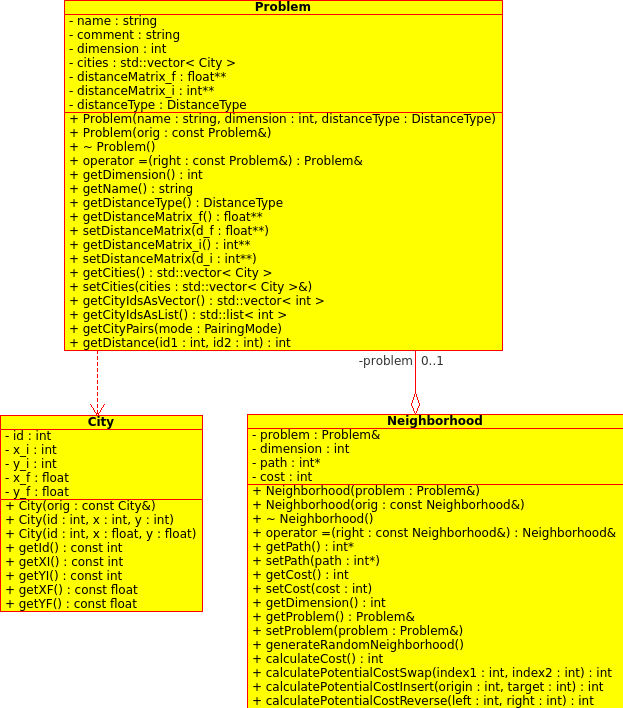
\includegraphics[width=\textwidth]{../UML/core.png}

\paragraph{}
\textbf{Problem} contient une matrice de distance, calculée une fois que toutes
les citées ont été enregistrées, qui va être l'attribut le plus important de
\textbf{Problem}, réutilisé par toutes les méthodes de calcul de coût.

\section{relation}
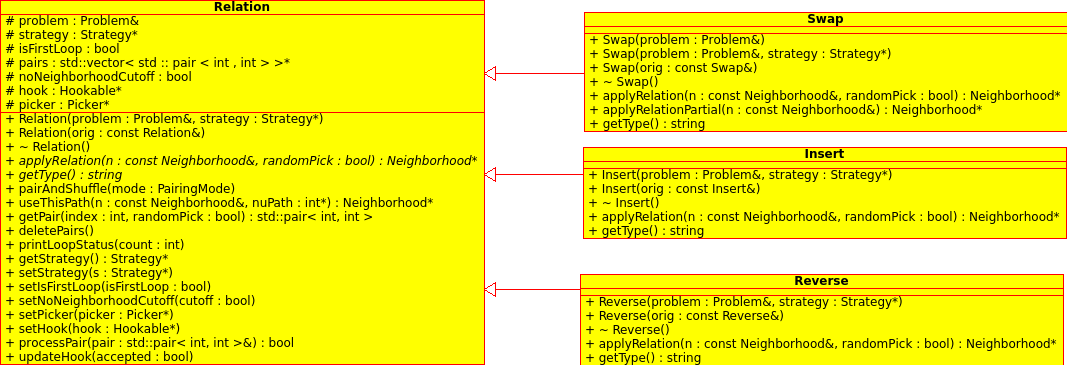
\includegraphics[width=\textwidth]{../UML/relation.png}

\section{strategy}
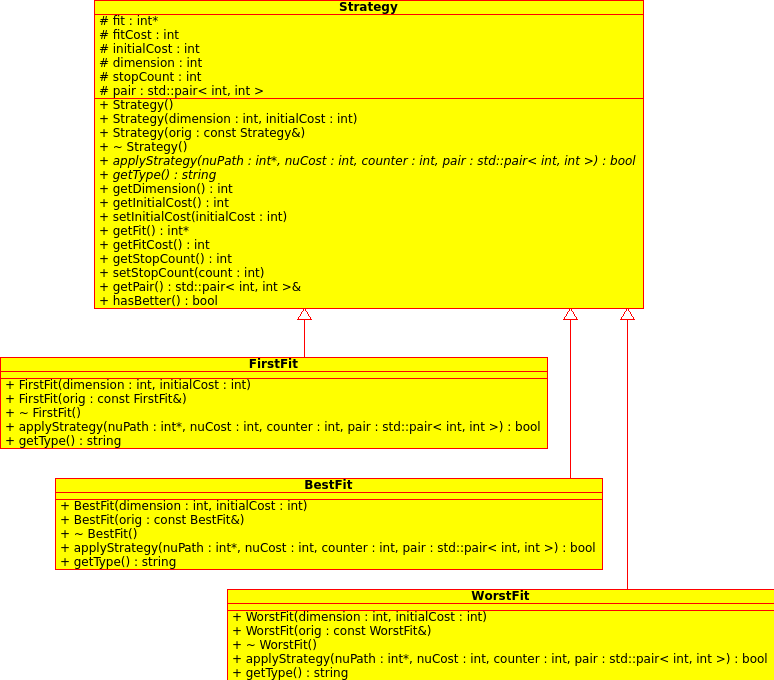
\includegraphics[width=\textwidth]{../UML/strategy.png}

\section{run}
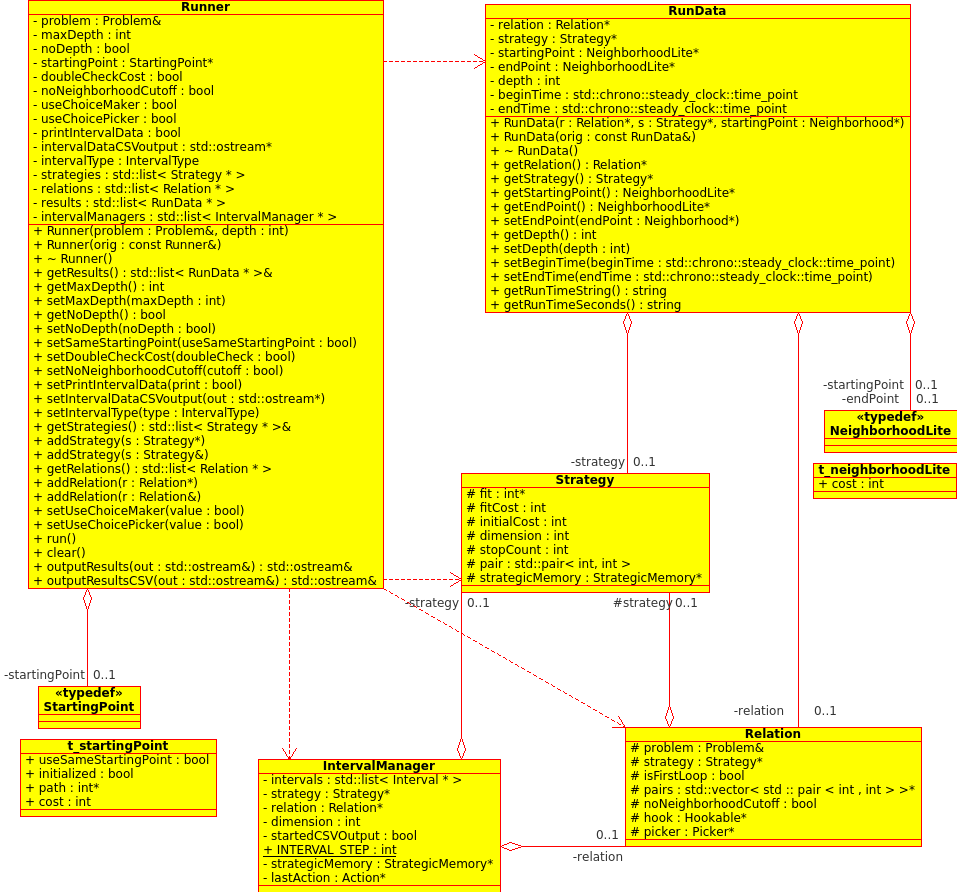
\includegraphics[width=\textwidth]{../UML/run.png}

\subsection{interval}
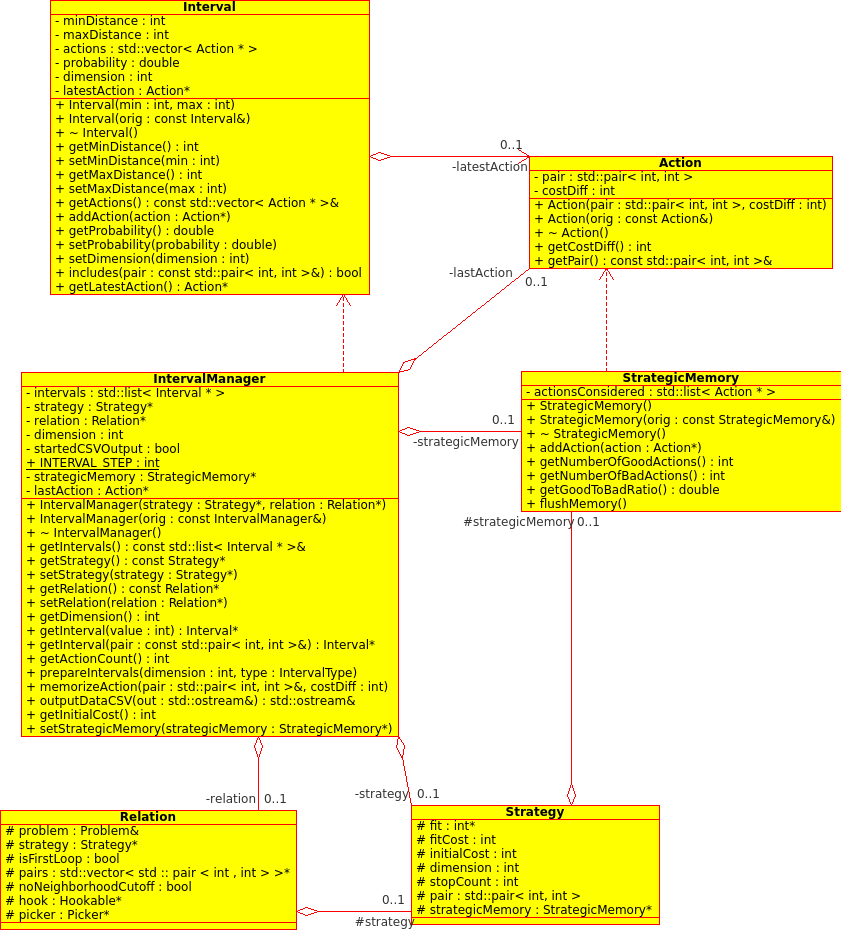
\includegraphics[width=\textwidth]{../UML/interval.png}

\section{hook}
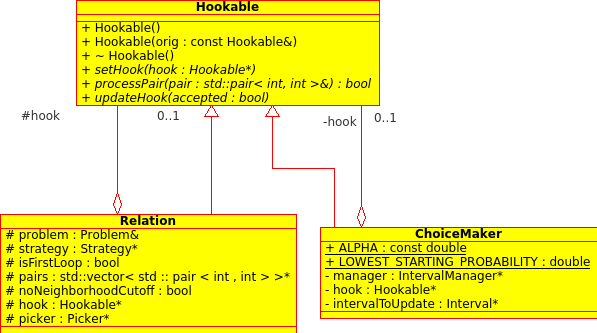
\includegraphics[width=\textwidth]{../UML/hook.png}

\section{choice}
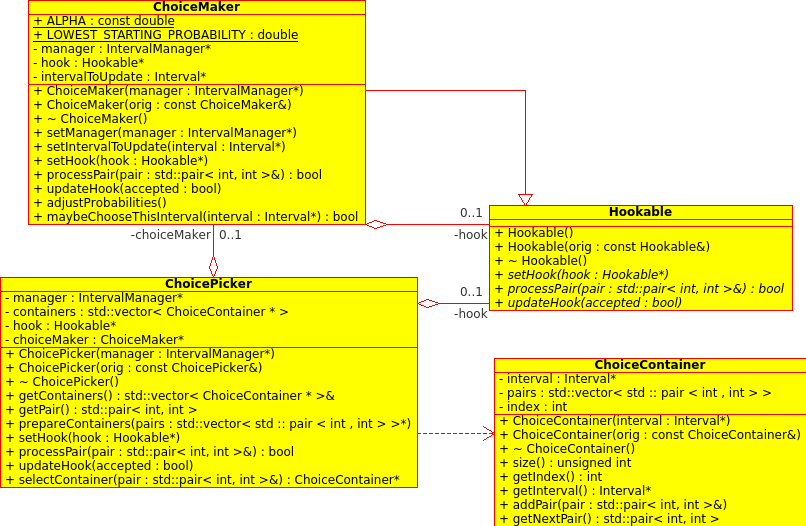
\includegraphics[width=\textwidth]{../UML/choice.png}

\chapter{Extraits de code}

\chapter{Résultats d'exécution}

\section{recap.ods}
\subsection{summary sheet}

%screens + description

\subsection{interval sheets}

%screens + description

\end{document}          
